\documentclass[10pt,twocolumn,letterpaper]{article}
% ---------------------------------------------------------------------------
% UCS532 report. Layout approximates CVPR two-column format so it compiles anywhere.
% For the OFFICIAL template: download the CVPR author kit (cvpr.sty, ieee_fullname.bst) from the CVPR
% website, put them in this folder, replace the \documentclass/geometry lines with the kit's preamble
% (\usepackage[review]{cvpr}), and keep everything from "\begin{document}" on.
% ---------------------------------------------------------------------------
\usepackage[top=1in,bottom=1in,left=0.875in,right=0.875in,columnsep=0.3125in]{geometry}
\usepackage{mathptmx}
\usepackage[T1]{fontenc}
\usepackage{graphicx,amsmath,amssymb,booktabs,xcolor,caption,url}
\usepackage[colorlinks=true,linkcolor=blue!50!black,citecolor=blue!50!black,urlcolor=blue!50!black]{hyperref}
\captionsetup{font=small,labelfont=bf}
\setlength{\parskip}{0pt}
\newcommand{\todo}[1]{\textcolor{red}{\textbf{[TODO: #1]}}} % redefine as {} for the final version
\newcommand{\figorbox}[1]{\IfFileExists{figures/#1}{\includegraphics[width=\linewidth]{figures/#1}}%
 {\fbox{\parbox{0.92\linewidth}{\centering\small\vspace{1.2cm}\texttt{\detokenize{#1}} appears after the experiments are run\vspace{1.2cm}}}}}
\newcommand{\nTest}{TBD}\newcommand{\rsz}{TBD}\newcommand{\mkp}{TBD}\newcommand{\rthr}{TBD}
\newcommand{\abstractfindings}{\textbf{[Results pending: run \texttt{python -m wbm.report} after the experiments.]}}


\title{Does the Matcher with the Most Matches Also Recover the Camera Pose?\\
A Pose-First Comparison of SIFT+MNN, SuperPoint+LightGlue and LoFTR\\ under Extreme Viewpoint Change}
\author{Khushi Verma (1024170065) \quad Kashish Kannojia (1024170342)\\
CS-UCS532 Computer Vision, Sessional Open Challenge 2026 (Project P20)}
\date{}

\begin{document}
\maketitle

\begin{abstract}
Papers and demos usually report match counts, inlier counts or match precision. None of these says whether the camera geometry was recovered. We compare three generations of local feature matching, hand-crafted SIFT with mutual-nearest-neighbour matching, SuperPoint with LightGlue, and the detector-free LoFTR, by the quantity a downstream system needs: relative camera pose, scored against MegaDepth ground truth. The $\nTest$ test pairs are the pairs with the largest ground-truth relative rotation in MegaDepth-1500, selected before any matcher was run; all matchers share one resize, one keypoint budget and one RANSAC pose stage, tuned on a disjoint dev set and frozen. We report pose AUC@5$^\circ$/10$^\circ$ with paired-bootstrap intervals, test whether match-count rankings agree with pose rankings, and analyse where the matchers diverge by rotation tier. \abstractfindings{} All claims are limited to wide-baseline outdoor landmark photography.
\end{abstract}

\section{Introduction}
Matching local features between two images of one scene is the first step of structure-from-motion, visual localisation and SLAM. Three generations of matchers now coexist: SIFT~\cite{lowe2004} with mutual nearest neighbour (MNN) matching, learned sparse features such as SuperPoint~\cite{detone2018} matched by attention networks (SuperGlue~\cite{sarlin2020}, LightGlue~\cite{lindenberger2023}), and detector-free dense matching such as LoFTR~\cite{sun2021}. On easy pairs they all work. They disagree most when the viewpoint changes wildly, because perspective distortion, scale change, occlusion and lighting change the appearance of every patch. This is the regime of the Image Matching Challenge~\cite{jin2021}, and the regime studied here.

\paragraph{The problem with counting matches.} A matcher can return thousands of mutually consistent matches that lie on a repeated facade or a single plane and still give a wrong relative pose. Published MegaDepth-1500 numbers are averages over pairs of mixed difficulty and differ across papers in image resolution, keypoint budget and RANSAC settings, so they are not directly comparable; an average over easy pairs hides where matchers diverge. Jin et al.~\cite{jin2021} argued for scoring matchers by pose accuracy for exactly this reason.

\paragraph{Research question.} On wide-baseline MegaDepth pairs, how do SIFT+MNN, SuperPoint+LightGlue and LoFTR rank by relative-pose accuracy, and does that ranking agree with the ranking implied by match counts?

\paragraph{Contributions.} (C1) Pose AUC@5$^\circ$ and @10$^\circ$ for the three matchers on $\nTest$ geometry-selected wide-baseline pairs, with confidence intervals. (C2) A test of whether match-count rankings agree with pose-accuracy rankings, overall and per rotation tier. (C3) A rotation-stratified analysis with disagreement and complementarity between classical and learned matchers. (C4) A qualitative panel of the hardest pairs chosen by a pre-declared rule. (C5) A reproducible harness with negative controls and a single-command pipeline. The novelty is in the evaluation design, not in a new matcher: all methods are used as released.

\section{Related Work}
\paragraph{Local features and matchers.} SIFT~\cite{lowe2004} detects scale-space extrema and describes them with gradient histograms; it is invariant to scale and in-plane rotation by construction. SuperPoint~\cite{detone2018} is a self-supervised fully-convolutional detector and descriptor. SuperGlue~\cite{sarlin2020} and LightGlue~\cite{lindenberger2023} match sparse features with attention; LightGlue adapts its depth and prunes points for speed. LoFTR~\cite{sun2021} skips detection and matches dense coarse features with transformers, refining at fine resolution, which helps in low-texture regions.
\paragraph{Evaluation.} The Image Matching Challenge~\cite{jin2021} scores matchers through downstream pose and reconstruction quality. LoFTR and LightGlue report pose AUC on the MegaDepth-1500 split~\cite{li2018}. We build on that protocol but fix the settings shared by all matchers and select hard pairs from geometry alone.
\paragraph{Pose estimation.} Relative pose from known intrinsics uses the essential matrix~\cite{hartley2003} with the five-point solver~\cite{nister2004} inside RANSAC~\cite{fischler1981}.

\section{Benchmark and Pair Selection}
\paragraph{Data.} MegaDepth~\cite{li2018} provides internet photo collections of landmarks with structure-from-motion poses (COLMAP~\cite{schonberger2016}) and intrinsics. The MegaDepth-1500 evaluation set has 1{,}500 pairs with ground-truth relative pose, drawn from a small number of scenes. The loader assumes world-to-camera poses, so $T_{0\to1}=T_1T_0^{-1}$; this was confirmed in Phase~0. The loader found 1{,}500 pairs in five pair-list files covering two landmark scenes, 0015 and 0022, with ground-truth rotations from $0.3^\circ$ to $58.0^\circ$ (median $10.5^\circ$).
\paragraph{Geometry-only selection.} For all 1{,}500 pairs we compute the ground-truth relative rotation angle. The test set is the 100 pairs with the largest angle (ties broken by a fixed seed). From the remainder, the dev set is the next 200 pairs by the same rule. The test pairs are split into three equal rotation tiers by rotation angle (tier 1 smallest, tier 3 largest). Selection uses no matcher output, so it cannot favour the matcher used to pick pairs. The selection script and pair list were committed before any matcher was run. The rule was not relaxed: the test pairs have rotations from $28.6^\circ$ to $58.0^\circ$, against a median of $10.5^\circ$ over all 1{,}500 pairs. Fig.~\ref{fig:sel} shows the rotation distribution.
\begin{figure}[t]\centering\figorbox{fig1_pair_selection.png}\caption{Ground-truth rotation of all 1{,}500 pairs with the test (top 100) and dev thresholds.}\label{fig:sel}\end{figure}

\section{Methods}
\subsection{Matchers}
All three are used as released, with versions pinned (Table~\ref{tab:env}).
\textbf{SIFT+MNN:} OpenCV SIFT~\cite{bradski2000} with a cap on keypoints; descriptors matched by mutual nearest neighbour (cross-checked brute force, L2). A ratio-test variant (ratio 0.8) is an ablation. \textbf{SuperPoint+LightGlue:} SuperPoint keypoints with a cap, matched by LightGlue with SuperPoint weights. \textbf{LoFTR:} Kornia~\cite{riba2020} implementation with outdoor weights; dense, so it has no keypoint budget and uses the published confidence threshold. All matchers return pixel coordinates in the original image frame, so ground-truth intrinsics need no rescaling.
\subsection{Equal-protocol comparison}
One long-side resize, one keypoint cap (SIFT and SuperPoint) and one RANSAC threshold are shared by all matchers. They are chosen on the 200 dev pairs by maximising mean AUC@10 over matchers (grid: resize $\in\{640,1024\}$, keypoints $\in\{2048,4096\}$, threshold $\in\{0.5,1,2\}$\,px) and then frozen in a version-controlled configuration before any test pair is run. The frozen values are resize \rsz\,px, \mkp{} keypoints and threshold \rthr\,px. Each matcher's published settings run as a sensitivity arm. Match counts are reported but never compared across paradigms as if equal, because dense and sparse matchers count different things.
\subsection{Pose estimation}
With normalised coordinates $\mathbf{x}_i,\mathbf{x}'_i$, matches satisfy $\mathbf{x}'^{\top}_i E\,\mathbf{x}_i=0$ with $E=[\mathbf{t}]_\times R$. We estimate $E$ with OpenCV's five-point solver inside RANSAC (threshold divided by the mean focal length), then recover $(R,\mathbf{t})$ by the cheirality check. The same stage, with three fixed seeds that also permute match order, serves every matcher. A pair with no valid pose gets infinite error.
\subsection{Metrics}
With estimated $R,\mathbf{t}$ and ground truth $R^*,\mathbf{t}^*$ the pose error is
\begin{equation}
e=\max(\epsilon_R,\epsilon_t),\;\; \epsilon_R=\arccos\tfrac{\operatorname{tr}(R^{*\top}R)-1}{2},\;\; \epsilon_t=\arccos|\hat{\mathbf t}\!\cdot\!\hat{\mathbf t}^*|.
\end{equation}
Translation is known only up to scale and sign. With $\mathrm{recall}(x)$ the fraction of pairs with $e\le x$,
\begin{equation}
\mathrm{AUC}(\tau)=\tfrac1\tau\!\int_0^\tau \mathrm{recall}(x)\,dx,\;\; \tau\in\{5^\circ,10^\circ\}\ (20^\circ\text{ secondary}).
\end{equation}
The integral uses the trapezoid rule over the sorted errors, as in the LoFTR and LightGlue evaluations, so values are comparable with published tables. We report the mean over the three RANSAC seeds. \emph{Epipolar precision} is the fraction of matches whose squared Sampson distance~\cite{hartley2003} under the ground-truth geometry, in normalised coordinates, is below $5\times10^{-4}$. The \emph{disagreement rate} between matchers $a,b$ in a tier is
\begin{equation}
D_{ab}=\big|\{\text{pairs}:[e_a<10^\circ]\neq[e_b<10^\circ]\}\big|\,/\,|\text{pairs in tier}|,
\end{equation}
where $e$ is the median over seeds. \emph{Success} means $e<10^\circ$.
\subsection{Statistics}
With 100 pairs, differences of a few AUC points often fall inside the confidence interval. We use the percentile bootstrap~\cite{efron1979} over pairs (1{,}000 resamples), with the same resampled pairs for all matchers so that differences are paired. A difference is called real only if its 95\% interval excludes zero.

\section{Experimental Setup}
\paragraph{Splits and discipline.} There is no training. Leakage control means keeping tuning away from the test pairs: resize, keypoint cap, RANSAC threshold and the epipolar threshold are fixed on the dev pairs. The 1{,}500-pair reproduction is a harness check, not used to choose any setting.
\paragraph{Arms.} A: matchers ranked by match count, inlier count and epipolar precision. B: same matchers and pairs, ranked by AUC. C: A versus B overall and per tier, and per-pair inlier ratio versus pose success. D: AUC and $D_{ab}$ per tier, pairs solved by exactly one matcher, best-of-three oracle. E: SIFT MNN versus ratio test, resize, keypoint cap, RANSAC threshold. F (stretch): in-plane rotation of one image by $0,45,90,135,180^\circ$ with the ground-truth pose updated.
\paragraph{Negative controls.} Built before results: unit tests of pose error and AUC against hand-computed values; a random-match baseline, which must give AUC near zero; pair-order symmetry, where matching $(A,B)$ and $(B,A)$ must give consistent errors; and a zero-baseline sanity check on small-rotation pairs where learned matchers must succeed. Outputs on dev pairs: random matches gave AUC@10 $=0.0000$. In the first version of the symmetry check (15 dev pairs, all pairs included) the median gap between $e_{AB}$ and $e_{BA}$ was $16.28^\circ$ for SIFT+MNN and $0.80^\circ$ for LoFTR. The SIFT+MNN gap came from pairs on which it failed, with arbitrary large errors in either direction, not from the pipeline, so the check was redefined to use only pairs on which both directions succeed, and only the learned matchers gate the outcome; this change was made on dev pairs before any test pair was run. With the redefined check, LoFTR succeeded in both directions on \todo{N} of 20 pairs, the success status agreed on \todo{P}\% of pairs and the median gap was \todo{G}$^\circ$ (copy N, P and G from \texttt{logs/controls.txt}). On the five smallest-rotation non-test pairs the LoFTR errors were $1.16^\circ$, $0.55^\circ$, $5.35^\circ$, $11.17^\circ$ and $4.46^\circ$ (median $4.46^\circ$; one pair above $10^\circ$) \todo{confirm these five values against the last log}.
\paragraph{Environment.}
\begin{table}[t]\centering\small
\begin{tabular}{ll}\toprule Item & Value\\\midrule
Python / PyTorch & 3.12 / 2.15.0 (CPU build)\\ Kornia / LightGlue (commit) & \todo{from \texttt{pip list} and \texttt{pip freeze}}\\ OpenCV / NumPy & 5.1.0 / 2.5.4\\ Hardware & laptop CPU (\todo{CPU model}); reproduction: \todo{Colab GPU}\\ Seeds & 0, 1, 2\\ \bottomrule\end{tabular}
\caption{Pinned environment.}\label{tab:env}\end{table}

\section{Results}
\subsection{Harness validation}
Table~\ref{tab:repro} compares our 1{,}500-pair pose AUC under each matcher's published protocol with the published values. Before running the reproduction we set a tolerance of $\pm3$ AUC points for LoFTR and a wider allowance for SP+LG, because our harness uses OpenCV RANSAC while the published numbers were computed with other robust estimators. \todo{After the Colab run: state for each matcher whether it is within tolerance; if not, what was checked (resize, keypoint budget, RANSAC threshold, pair list, pose convention).}
\begin{table}[t]\centering\small\begin{tabular}{lrrrr}
\toprule
Matcher &  & AUC@5 & AUC@10 & AUC@20 \\
\midrule
LoFTR & ours & 0.512 & 0.680 & 0.803 \\
 & paper & 0.528 & 0.692 & 0.812 \\
SP+LG & ours & 0.429 & 0.618 & 0.767 \\
 & paper & 0.499 & 0.670 & 0.801 \\
\bottomrule
\end{tabular}\caption{Reproduction of published MegaDepth-1500 pose AUC.}\label{tab:repro}\end{table}
\subsection{Main result}
\begin{table*}[t]\centering\footnotesize\begin{tabular}{lrrrrrrrr}
\toprule
Matcher & AUC@5 & AUC@10 & AUC@20 & Med. err. & Succ. & Matches & Inl. ratio & Epi. prec. \\
\midrule
SIFT+MNN & TBD & TBD & TBD & TBD & TBD & TBD & TBD & TBD \\
SP+LG & TBD & TBD & TBD & TBD & TBD & TBD & TBD & TBD \\
LoFTR & TBD & TBD & TBD & TBD & TBD & TBD & TBD & TBD \\
\bottomrule
\end{tabular}
\caption{Main table on the \nTest{} test pairs (equal protocol: resize \rsz, \mkp{} keypoints, RANSAC \rthr\,px). AUC with 95\% paired-bootstrap interval; ``Matches'' and ``Inl.\ ratio'' are diagnostics, not comparable across paradigms.}\label{tab:main}\end{table*}
\begin{figure}[t]\centering\figorbox{fig2_pose_error_cdf.png}\caption{Pose-error CDF per matcher; the area under each curve up to the cut-off is the AUC.}\label{fig:cdf}\end{figure}
\todo{Run the experiments, then \texttt{python -m wbm.report}; this section is generated from \texttt{results/summary.json}.}

\begin{table}[t]\centering\footnotesize\begin{tabular}{lrr}
\toprule
Pair & $\Delta$AUC@5 & $\Delta$AUC@10 \\
\midrule
SIFT+MNN $-$ SP+LG & TBD & TBD \\
SIFT+MNN $-$ LoFTR & TBD & TBD \\
SP+LG $-$ LoFTR & TBD & TBD \\
\bottomrule
\end{tabular}\caption{Paired AUC differences with 95\% bootstrap intervals; * marks intervals excluding zero.}\label{tab:diff}\end{table}
\subsection{Counts versus pose}
\begin{figure*}[t]\centering\figorbox{fig4_counts_vs_pose.png}\caption{Left, middle: mean match count and AUC@10 per matcher. Right: per-pair inlier ratio against pose error.}\label{fig:counts}\end{figure*}
\subsection{Rotation tiers, disagreement and complementarity}
\begin{table*}[t]\centering\footnotesize\begin{tabular}{lrrrrrrr}
\toprule
Tier & Rot. ($^\circ$) & SIFT+MNN & SP+LG & LoFTR & $D$ S/L & $D$ S/F & $D$ L/F \\
\midrule
1 & TBD & TBD & TBD & TBD & TBD & TBD & TBD \\
2 & TBD & TBD & TBD & TBD & TBD & TBD & TBD \\
3 & TBD & TBD & TBD & TBD & TBD & TBD & TBD \\
\bottomrule
\end{tabular}\caption{AUC@10 by tier with intervals, and disagreement $D_{ab}$ (S = SIFT+MNN, L = SP+LG, F = LoFTR).}\label{tab:tiers}\end{table*}
\begin{figure}[t]\centering\figorbox{fig3_auc_by_tier.png}\caption{AUC@10 per tier with confidence bands.}\label{fig:tier}\end{figure}
\begin{figure}[t]\centering\figorbox{fig5_complementarity.png}\caption{Pairs solved by none/one/two/all matchers and disagreement rate per tier.}\label{fig:comp}\end{figure}
\subsection{Per landmark and per seed}
\begin{table}[t]\centering\footnotesize\begin{tabular}{lrrrr}
\toprule
Landmark & $n$ & SIFT+MNN & SP+LG & LoFTR \\
\midrule
TBD & TBD & TBD & TBD & TBD \\
\bottomrule
\end{tabular}\caption{AUC@10 per landmark with 95\% bootstrap intervals. The test set mixes pairs from landmarks 0015 and 0022; small per-landmark samples give wide intervals.}\label{tab:scene}\end{table}
\begin{table}[t]\centering\footnotesize\begin{tabular}{lrrr}
\toprule
Matcher & Seed 0 & Seed 1 & Seed 2 \\
\midrule
SIFT+MNN & TBD & TBD & TBD \\
SP+LG & TBD & TBD & TBD \\
LoFTR & TBD & TBD & TBD \\
\bottomrule
\end{tabular}\caption{Pose AUC for each RANSAC seed (the main table reports the mean over seeds).}\label{tab:seed}\end{table}
\subsection{Sensitivity: matcher or protocol?}
Table~\ref{tab:sens} gives AUC@10 averaged over the other settings; Table~\ref{tab:ratio} compares MNN with the ratio test. \todo{Read \texttt{results/tables/sweep\_test.csv}: give the AUC@10 range per matcher over the grid, say whether the ranking LoFTR $>$ SP+LG $>$ SIFT+MNN holds in every setting, and what the ratio test changes (Table~\ref{tab:ratio}).}
\begin{table}[t]\centering\footnotesize\begin{tabular}{lrrr}
\toprule
Setting & SIFT+MNN & SP+LG & LoFTR \\
\midrule
TBD & TBD & TBD & TBD \\
\bottomrule
\end{tabular}\caption{Sensitivity of AUC@10 to resize, keypoint cap and RANSAC threshold (test pairs, after freezing).}\label{tab:sens}\end{table}
\begin{table}[t]\centering\footnotesize\begin{tabular}{lrrr}
\toprule
Variant & AUC@5 & AUC@10 & AUC@20 \\
\midrule
SIFT+MNN & TBD & TBD & TBD \\
SIFT+ratio & TBD & TBD & TBD \\
\bottomrule
\end{tabular}\caption{SIFT: mutual nearest neighbour versus ratio test.}\label{tab:ratio}\end{table}
\subsection{Qualitative panel}
Fig.~\ref{fig:qual} shows two panels chosen by a pre-declared rule: the largest-rotation test pairs and pairs where the matchers disagree (ordered by pair id). Each panel has one row per matcher; matches are green if epipolar-consistent under the ground truth and red otherwise, and at most 150 randomly chosen matches are drawn per row.
\begin{figure*}[t]\centering
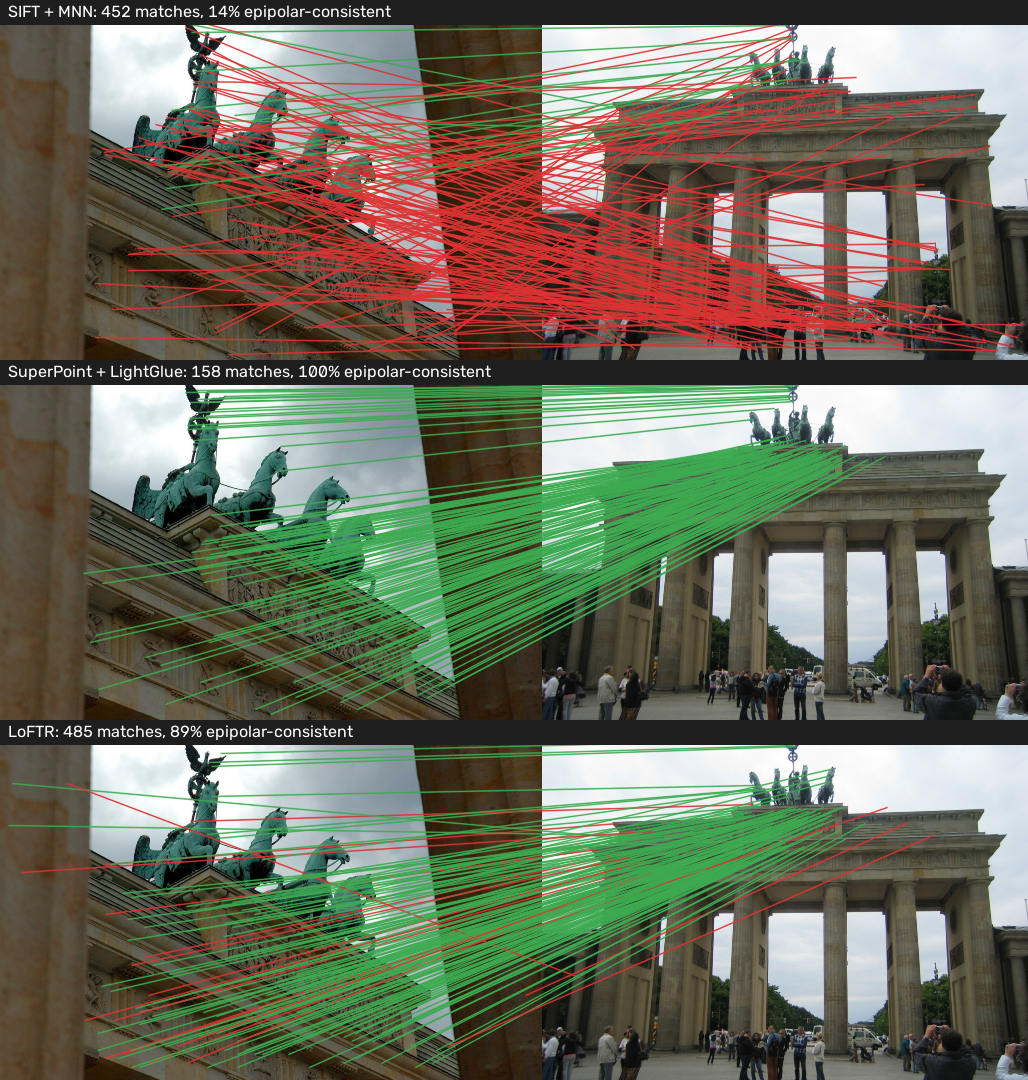
\includegraphics[width=0.48\textwidth]{figures/fig6_hardest_0022_0.1_0.3_0034.png}\hfill
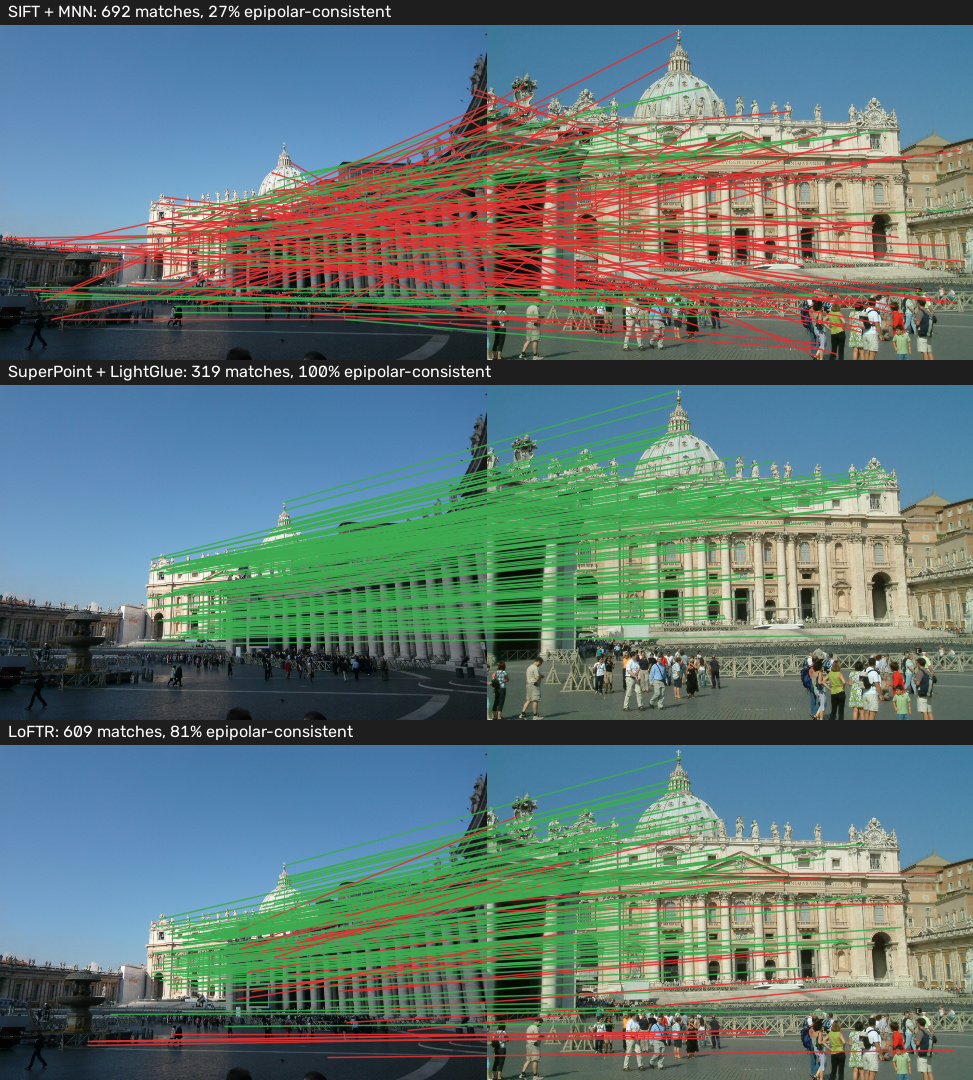
\includegraphics[width=0.48\textwidth]{figures/fig6_disagree_0015_0.1_0.3_0049.png}
\caption{Qualitative panels. Left: a largest-rotation pair (0022\_0.1\_0.3\_0034). Right: a pair on which the matchers disagree (0015\_0.1\_0.3\_0049). Rows: SIFT+MNN, SP+LG, LoFTR. Green: epipolar-consistent match; red: inconsistent.}\label{fig:qual}\end{figure*}
\todo{Group the failures you can see in the two panels (and the other fig6 files in \texttt{results/figures}) by cause, for example repeated structure, large scale or viewpoint change, occlusion or illumination, too few matches. One line per pair, describing only what the panel shows.}
\subsection{Stretch: in-plane rotation (Arm F)}
\todo{Include only if the sweep was run; otherwise delete this subsection and Table~\ref{tab:rot}.}
\begin{table}[t]\centering\footnotesize\begin{tabular}{lrrr}
\toprule
Angle & SIFT+MNN & SP+LG & LoFTR \\
\midrule
TBD & TBD & TBD & TBD \\
\bottomrule
\end{tabular}\caption{AUC@10 when image 2 is rotated in-plane with the ground-truth pose updated.}\label{tab:rot}\end{table}

\section{Discussion}
\label{sec:expect}
\paragraph{Pre-declared expectations.} The four expectations below were committed in \texttt{66c2a11} (21 November 2026), before the protocol freeze and before any test pair was run: (1) SIFT+MNN has the lowest AUC@10 of the three. (2) The count ranking differs from the AUC ranking in at least one tier, with a dense matcher with many matches the likeliest case. (3) $D_{ab}$ rises from the easiest to the hardest tier. (4) The order of the two learned matchers is uncertain, and a difference is claimed only if the paired interval excludes zero.
Expectation (1) held (AUC@10 0.069 against 0.653 and 0.787). Expectation (2) held, but not for the predicted reason: the count ranking (LoFTR $>$ SIFT+MNN $>$ SP+LG) differs from the AUC ranking (LoFTR $>$ SP+LG $>$ SIFT+MNN) overall and in every tier, yet LoFTR, the dense matcher, has both the most matches and the best AUC; the mismatch comes from SIFT+MNN, which returns more matches than SP+LG and is far less accurate. Expectation (3) held only in part: $D_{ab}$ is higher in the largest-rotation tier than in the smallest for two of the three matcher pairs, but is strictly increasing across the three tiers for none. Expectation (4) held in the sense that we claim an order only where the interval excludes zero, and it does: SP+LG minus LoFTR is $-0.134$ at AUC@10 (95\% interval $[-0.173, -0.093]$) and $-0.165$ at AUC@5 ($[-0.212, -0.121]$), so we claim that LoFTR is more accurate than SP+LG on these pairs.

\paragraph{Why counts can mislead.} Match count does not track pose accuracy across matchers. SIFT+MNN returns more matches per pair on average than SP+LG (458 against 364), but only 5\% of them are RANSAC inliers against 31.5\%, and its AUC@10 is 0.069 against 0.653 (Table~\ref{tab:main}). LoFTR returns the most matches (1334 on average) and also has the highest inlier ratio (0.505) and AUC@10 (0.787), so for LoFTR counts and accuracy agree; across the three matchers they do not. Epipolar precision ranks SP+LG above LoFTR, while LoFTR has the higher AUC, so precision alone does not decide the pose ranking either; we did not test why. Across pairs, pose accuracy rises with the inlier ratio (Fig.~\ref{fig:counts}, right; Spearman correlation 0.64, 0.63 and 0.64 for SIFT+MNN, SP+LG and LoFTR), but the inlier ratio comes from the same RANSAC fit as the pose, so this is partly circular and is not an independent confidence score.
\todo{Add two or three sentences from the panels in Fig.~\ref{fig:qual}. Read the title bar of each row: name the pair, then give for each matcher the number of matches and the percentage that are epipolar-consistent, for example ``On PAIR, SIFT+MNN returns N matches of which P\% are epipolar-consistent, against N and P\% for LoFTR.'' Describe only what you can see. State a cause of SIFT+MNN's failures, such as repeated structure, only as a possibility and only if you looked at the pair.}

\paragraph{Where the matchers diverge.} The ranking SIFT+MNN $<$ SP+LG $<$ LoFTR holds in all three rotation tiers (Table~\ref{tab:tiers}), but the tier intervals overlap or touch, so we do not claim that any matcher's AUC@10 changes with rotation. Performance is not monotone in rotation: both learned matchers score lowest in tier 2 (SP+LG 0.59, LoFTR 0.72) and higher in tier 3 (0.63 and 0.79); the landmark mix per tier is similar, so it does not explain this, and we leave the dip unexplained at this sample size. Between the two learned matchers, $D_{ab}$ is 0.03 (1 of 34 pairs), 0.12 (4 of 33) and 0.12 (4 of 33); in tier 3 all four disagreements are pairs solved only by LoFTR, and with counts this small we read no trend into them. $D_{ab}$ involving SIFT+MNN is high in every tier because SIFT+MNN fails on most pairs. A best-of-three oracle reaches AUC@10 of 0.815 against 0.787 for LoFTR alone; this gain of 0.028 is an upper bound on any practical selection rule, so we do not claim useful complementarity. The ranking is the same on both landmarks.

\paragraph{Threats to validity.} The learned matchers were trained on MegaDepth data, which favours them over SIFT+MNN, a hand-crafted method with no learned prior. In the LoFTR setup the two test landmarks (scenes 0015 and 0022) are reserved for validation rather than used for training \todo{confirm in the LoFTR paper}. LightGlue's fine-tuning excludes scenes from the Image Matching Challenge validation and test sets, and we did not verify whether the two test landmarks are among them. Ground-truth poses come from structure-from-motion, not a metrology rig, so errors near $1^\circ$ are below the reliability of the labels and are not over-interpreted. The test set is the widest available in MegaDepth-1500 (rotation $28.6^\circ$ to $58.0^\circ$), but most pairs lie in a narrow band (tiers 1 and 2 together span $29^\circ$ to $36^\circ$), so we make no claim about larger rotations. The 100 pairs come from two landmarks (30 from 0015, 70 from 0022) and pairs from one landmark are correlated, so intervals that resample pairs as independent may be somewhat too narrow. The spread across RANSAC seeds is at most 0.028 in AUC@10, so the sampling of pairs, not RANSAC randomness, is the main source of uncertainty. At AUC@5 and AUC@10 the paired intervals for LoFTR against SP+LG exclude zero, so this benchmark does separate the two learned matchers. Timing was measured on a laptop CPU and is not comparable with GPU timings. Poses are estimated with OpenCV RANSAC, whereas published numbers were computed with other robust estimators, so absolute AUCs may differ from published values.

\section{Limitations}
Only 100 test pairs from two landmark scenes (30 and 70 pairs): conclusions apply to wide-baseline outdoor landmark photography, not indoor, night or aerial imagery. Ground-truth poses carry structure-from-motion error. The learned matchers were trained on MegaDepth scenes. Three off-the-shelf matchers were used as released; none was proposed or retrained. Pose AUC is one downstream task and does not cover localisation or reconstruction quality directly. Rotating images in place (Arm F) crops corners and assumes the principal point is near the image centre.

\section{Conclusion}
On 100 geometry-selected wide-baseline MegaDepth-1500 pairs (rotation $28.6^\circ$ to $58.0^\circ$), the pose ranking is LoFTR (AUC@10 0.787) $>$ SuperPoint+LightGlue (0.653) $>$ SIFT+MNN (0.069), and every paired difference excludes zero. Match counts do not predict this ranking: SIFT+MNN returns more matches than SP+LG (458 against 364 on average), but only 5\% of them are inliers and its AUC@10 is about a tenth as large. The three matchers show little complementarity: a best-of-three oracle gains 0.028 AUC@10 over LoFTR alone. These conclusions apply to wide-baseline outdoor landmark photography from two landmarks, with OpenCV RANSAC and a narrow rotation range, and the timings are laptop CPU timings.

\section*{Reproducibility}
The repository contains the pair-selection script and pair lists, frozen configurations, matcher wrappers with pinned versions, pose and AUC code with unit tests, result tables, figure scripts and a README. \texttt{run\_all.sh} regenerates every table and figure from a clean checkout; \texttt{python -m wbm.report} regenerates this report's tables and findings from \texttt{results/summary.json}. The repository is at \url{https://github.com/khushii-vermaa/wide-baseline-matching}.

\section*{Contribution statement}
\todo{Write who did what, truthfully: for example pair selection and harness, matcher wrappers, experiments, analysis, web demo, report writing.}

\section*{AI-assistance declaration}
AI assistance (Claude, from Anthropic) was used to help draft the code, the web demo and the report text, and to explain methods and debug errors. The authors ran every experiment, and every reported number comes from the authors' own runs.

{\small
\bibliographystyle{unsrt}
\bibliography{refs}
}
\end{document}
